\documentclass[12pt]{article}
\usepackage{fullpage,enumitem,amsmath,amssymb,graphicx, listings,cite}%,hyperref}

\usepackage{hyperref}
\usepackage{xcolor}
\hypersetup{
   colorlinks,
   linkcolor={red!50!black},
   citecolor={blue!50!black},
   urlcolor={blue!80!black}
}

\title{Enabling Affordable Precision Agriculture by Sensing Soil Moisture Wirelessly}
\author{Colleen Josephson\\Advised by:  Ranveer Chandra (Microsoft) and Sachin Katti (Stanford)}
%\date{the FUTURE!!!}
\begin{document}
\maketitle

\begin{abstract}
  The term ``precision agriculture'' has been around since the 1980s,
  and it describes a farming technique that uses extensive measurement
  of crop data to make informed decisions about watering,
  fertilization and more. Despite decades of work, precision
  agriculture is still not widely implemented on working farms. This
  is because the data is hard to collect and process, primarily due to
  the lack of high speed internet access in rural areas, and the high
  cost and difficulty of deploying dense sensor networks. Recent work
  such as Farmbeats~\cite{farmbeats} has made good progress in
  addressing the issues of internet access, but the cost and
  deployability of sensors remains an issue. We seek to address this
  by designing a low-cost and easy-to-use wireless soil moisture
  sensor.
\end{abstract}


\section*{Introduction}

Agriculture is the single largest pressure on the world's sources of
fresh water--- 69\% of the global fresh water supply is used for
agriculture~\cite{water}. Paired with the fact that the world's
population is projected to exceed 9 billion by 2050~\cite{population},
with most of the growth coming from developing nations in Africa,
conservation of fresh water and sufficient food production are key
concerns that need to be addressed. Soil moisture is the most
important measurement for ensuring the maximization of crop yield
without water waste.

Multiple studies show that soil moisture sensors lead to a water
savings of at least 20\%\cite{watersavings}, and in some cases more
than 50\%, while maintaining crop yields. Yet soil sensors are still
not widely deployed on working farms, despite decades of research
confirming the benefits. The lack of widespread adoption can be
attributed to a few key challenges: 1.) high sensor cost 2.)
difficulty of deploying and maintaining the sensors and 3.) difficulty
collecting and processing the sensor data.

The average commercial\footnote{People are often misled by the
  SparkFun soil moisture sensor retailing for \$6.95. This is just a
  raw sensor probe, with no wiring, weatherproofing, testing or
  calibration. The added cost of a power source, data logger and
  wiring is more than \$40, and the system is still not weatherproofed
  or calibrated.} soil moisture sensor is more than \$100, which does
not include the power source or data logger to record and/or transmit
the measurement samples. The cost is at least \$50 to add the cheapest
DIY weatherproof logger and transmitter.  Since soil is not uniform
across a field, nevermind an entire farm, multiple sensors are needed
to accurately measure moisture for irrigation purposes. The average
farm in the United States is 444 acres~\cite{farmsize}. The water cost
for a tomato farm of that size would be approximately \$55,000 per
year~\cite{agwater}~\cite{tomatoes}, which means a precision soil
moisture system would lead to \$11,000 in savings. However, the cost
of deploying 20 sensors~\cite{sensorDensity} per acre would more than
\$1,000,000 with today's sensor costs. The current high cost of
sensors makes it difficult to for the average farmer to justify
investing in precision agriculture. Furthermore, this cost makes soil
moisture sensing completely infeasible for small-holder farmers in
developing nations, which is where the most of the food and water
insecurity will be located.

On top of the high cost, current sensors are not simple to deploy and
maintain. Very few sellers offer a product that includes the sensor,
logger and power source ready for immediate use. Therefore some amount
of setup labor is required for each sensor. Figure 1 shows a typical
sensor and data logging system. Though the sensor is waterproof, the
data logger (in this case an Arduino) needs to be waterproofed and
powered. The soil moisture sensor needs to be burried, which requires
digging a hole to the desired depth. This project also attaches solar
panel to the battery pack, which requires mounting high enough to
harvest sunlight, probably requiring a wooden or metal post. The
laborious process of burying the sensor and mounting the solar panel
would need to be repated for every sensor node on the
farm. Furthermore, the excess cables and bulky box also make the
system easy to tangle in farm eqipment and tools. The sensor system
would need to gently removed and re-deployed every time the field is
tilled. This all adds up to a significant amount of manual labor to
deploy and maintain the soil moisture sensors.

\begin{figure*}[h!]
  \centering
  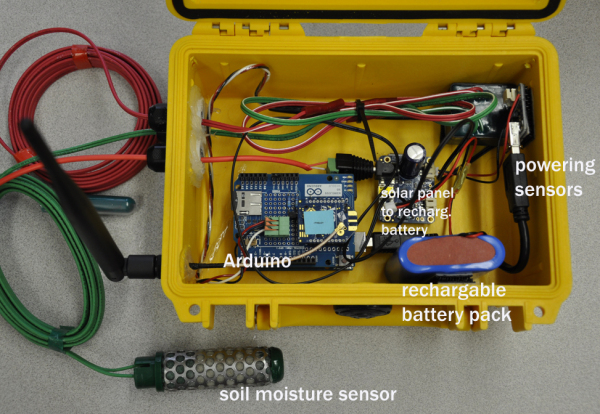
\includegraphics[scale=0.75]{soil_moisture_sn_setup.jpg}\\
  \caption{A weatherproofed soil moisture sensor box from the
    Geosensor Networks Lab~\cite{sensorbox}}
\end{figure*}

Finally, the data needs to be collected from the logger. For a 444
acre farm, the most practical method is wireless collection. Extending
wireless coverage to a large farm is not simple, especially because
cellular coverage in rural areas tends to be poor. A number of recent
works have considered the issue of networking sensors in rural
environments. For example, the 2015 Farmbeats project looks at the
issue of sensor data collection and network access extensively, using
TV whitespace technology to provide a wireless gateway from the field
to the Inernet. Though solving this challenge is also important, the
focus of our research will be on reducing the cost and improving the
deployability and maintainability of soil moisture sensors.

In the next section we will give an overview of current sensing
technology and related work.
    
\section*{Overview of sensing techniques}

There are three primary types of soil moisture sensors used in
agriculture: tensiometers, granular matrix sensors, and volumetric
sensors~\cite{sensorTypes}.

\subsubsection*{Tensiometers} Tensiometers measure soil water
tension. An air-free tube of water is attached to a porus tip, such as
ceramic. As water extracted from the soil by plants, the vacuum in the
tube increases. When the soil is irrigated, the pressure decreases. A
pressure sensor at the top of the tube is used to make the moisture
measurements. The response time to moisture changes is typically 2-3
hours. Tensiometers are slightly cheaper than the volumetric sensors
discussed earlier, but still require a dedicated data
logger/transmitter. They typcally require regular maintenance, such as
adding water or removing air from the tube. Tensiometers also only
operate when soils are relatively wet, and cannot be used when there
is any risk of freezing temperatures.

\subsubsection*{Granular matrix sensors (GMS)} Granular matrix sensors
measure electrical resistance in a porous medium like ceramic. As
water seeps into the porus medium, it reduces the electrical
resistance. The ceramic in GMSes naturally filter out ions from
fertilizer and salt, which would impact the resistance readings. GMSes
cost similar to tensiometers, but take longer to respond, do not work
well in very wet soil, and are more difficult to install. They do,
however, require significantly less maintenance.

\subsubsection*{Volumetric sensors}Volumetric sensors estimate
$\frac{V_{water}}{V_{wet soil}}$, the ratio of the volume of the water
to the volume of the soil plus the same volume of water. As the
volumetric water content changes, the dilectric permittivity constant
of the soil changes. Recall that dielectric permittivity,
$\varepsilon$, is the ability of a substance to hold an electrical
charge. The dielectric permittivty constant (also known as relative
permittivity), $\varepsilon_r$, is the ratio of the permittivity of
the stubstance to the permittivity of free space,
$\varepsilon_0$. Permittivity is often treated as a complex number:
$\varepsilon = \varepsilon' + j\varepsilon ''$, where $\varepsilon '$
is the real component and $\varepsilon''$ is the complex.

There are two main types of volumetric sensors: capacitive and time
domain refelectometry (TDR). Capacitive sensors measure the charge
time of a capacitor, which is a roughly linear function of
$\varepsilon$~\cite{sensorOverview}...

TDR sensors...(explain relation to GPR)

In 2017 researchers at Mircosoft Research figured out how to measure
soil moisture using consumer-grade WiFi signals...

\section*{Proposed approach}
-extremely low cost of RFID
-maintainable because the sensors are expendable
-advantages of radar backscatter over WiFi
-multi-depth sensors for cheap

\section*{Next steps}
\section*{Future work}
Environmental impact of tags
Leaf moisture
\section*{Conclusion}

\bibliographystyle{amsplain}
\begin{footnotesize}
\bibliography{soil_proposal}
\end{footnotesize}
\end{document}
